%%%%%%%%%%%%%%%%%%%%%%%%%%%
% PROBABILISTIC INVERSION %
%%%%%%%%%%%%%%%%%%%%%%%%%%%
The introduced Bayesian multilevel model \cref{eq:PEM:Multilevel:Model} acts as a toolkit for statistical model building.
It forms some kind of superstructure that embeds a variety of stochastic inverse problems as special cases.
In this section we will show how different well-known types of inverse problems are obtained by omitting global parameters and/or experiment-specific variables accordingly.
%%%%%%%%%%%%%%%%%%%%%%%%%%%%
\par % CLASSICAL INVERSION %
%%%%%%%%%%%%%%%%%%%%%%%%%%%%
\textit{Classical} or \textit{simple Bayesian inversion} is concerned with the estimation of fixed yet unknown parameters \(\bm{m}\) of the physical simulator \cite{Inversion:Tarantola2005,Inversion:Kaipio2005}.
% DAG
The related DAG is pictured in \cref{fig:PEM:DAG:SimpleInv}.
% ``SIMPLE''
In this context the term ``simple'' merely refers to the degree of sophistication of the input uncertainty model.
As a matter of fact classical inversion may not be a simple problem at all.
% NUMERICAL EXPENSE
It typically calls for a high number of forward solves.
The engineering community therefore relies on customized strategies in order to ameliorate the computational burden to Bayesian inference in real-case problems.
% ACCELERATION
This includes the employment of polynomial chaos expansions as forward model substitutes \cite{PCE:Marzouk2007,PCE:Marzouk2009:a,PCE:Tagade2014},
advanced stochastic simulation techniques \cite{MCMC:Beck2002,MCMC:Ching2007} and forward model reduction methods \cite{Bayesian:Papadimitriou2013,Bayesian:Jensen2014}.
%%%%%%%%%%%%%%%%%%%%%%%%%%%%%%%%
\par % PROBABILISTIC INVERSION %
%%%%%%%%%%%%%%%%%%%%%%%%%%%%%%%%
\textit{Probabilistic inversion} features a more elaborate two-level representation of input uncertainty \cite{Nagel:IPW2013:Proc,Multilevel:Ballesteros2014:Proc}.
Rather than aiming at an unknown constant \(\bm{m}\), inference concentrates on the hyperparameters \(\bm{\theta}_{\bm{X}}\)
that determine the variability of \(\tuple{\bm{x}_i}\) through \(f_{\bm{X} \cond \bm{\Theta}_{\bm{X}}} (\bm{x}_i \cond \bm{\theta}_{\bm{X}})\).
A DAG belonging to probabilistic inversion is depicted in \cref{fig:PEM:DAG:ProbInv}.
% ADDITIONAL NUISANCE
Building upon probabilistic inversion one may have variable inputs \(\tuple{\bm{\zeta}_i}\),
the distributions of which \(f_{\bm{Z}}(\bm{\zeta}_i \distparam \bm{\theta}_{\bm{Z}_i})\) are prescribed by \(\tuple{\bm{\theta}_{\bm{Z}_i}}\).
Unless experiment-specific realizations of those variables are of inferential interest, they act as additional nuisance parameters impeding the inference of the QoI.
The correspondingly extended DAG is provided in \cref{fig:PEM:DAG:AddPres}.
% NEARLY FULL FRAMEWORK
Of course, more complex modeling scenarios can be envisaged.
An application example where inference targets both parameters of the type \(\bm{m}\) and \(\bm{\theta}_{\bm{X}}\),
in the presence of additional nuisance parameters \(\tuple{\bm{\zeta}_i}\), can be found in \cite{Nagel:SciTech2014:Proc,Nagel:JAIS2015}.
% DAGS: SIMPLE & PROBABILISTIC INVERSION & ADDITIONAL PRESCRIPTION
\begin{figure}[ht]
  \centering
  \begin{subfigure}[b]{0.33\textwidth}
    \centering
    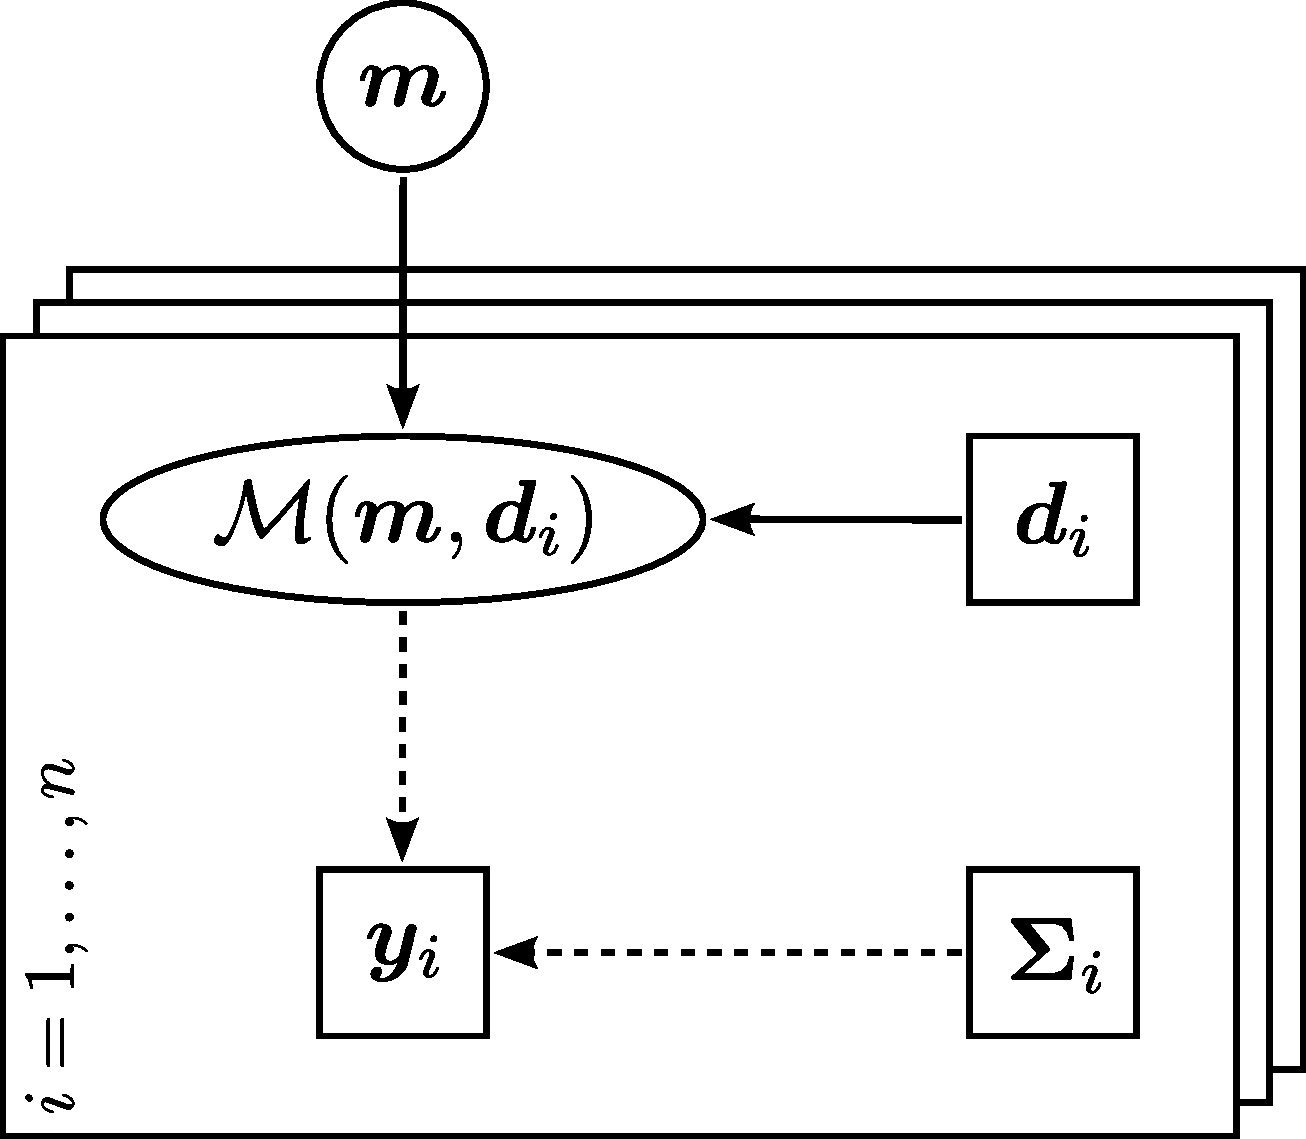
\includegraphics[width=\PEMdagWidth]{fig_PEM_DAG_SimpleInversion}
    \caption{Simple inversion.}
    \label{fig:PEM:DAG:SimpleInv}
  \end{subfigure}%
  \begin{subfigure}[b]{0.33\textwidth}
    \centering
    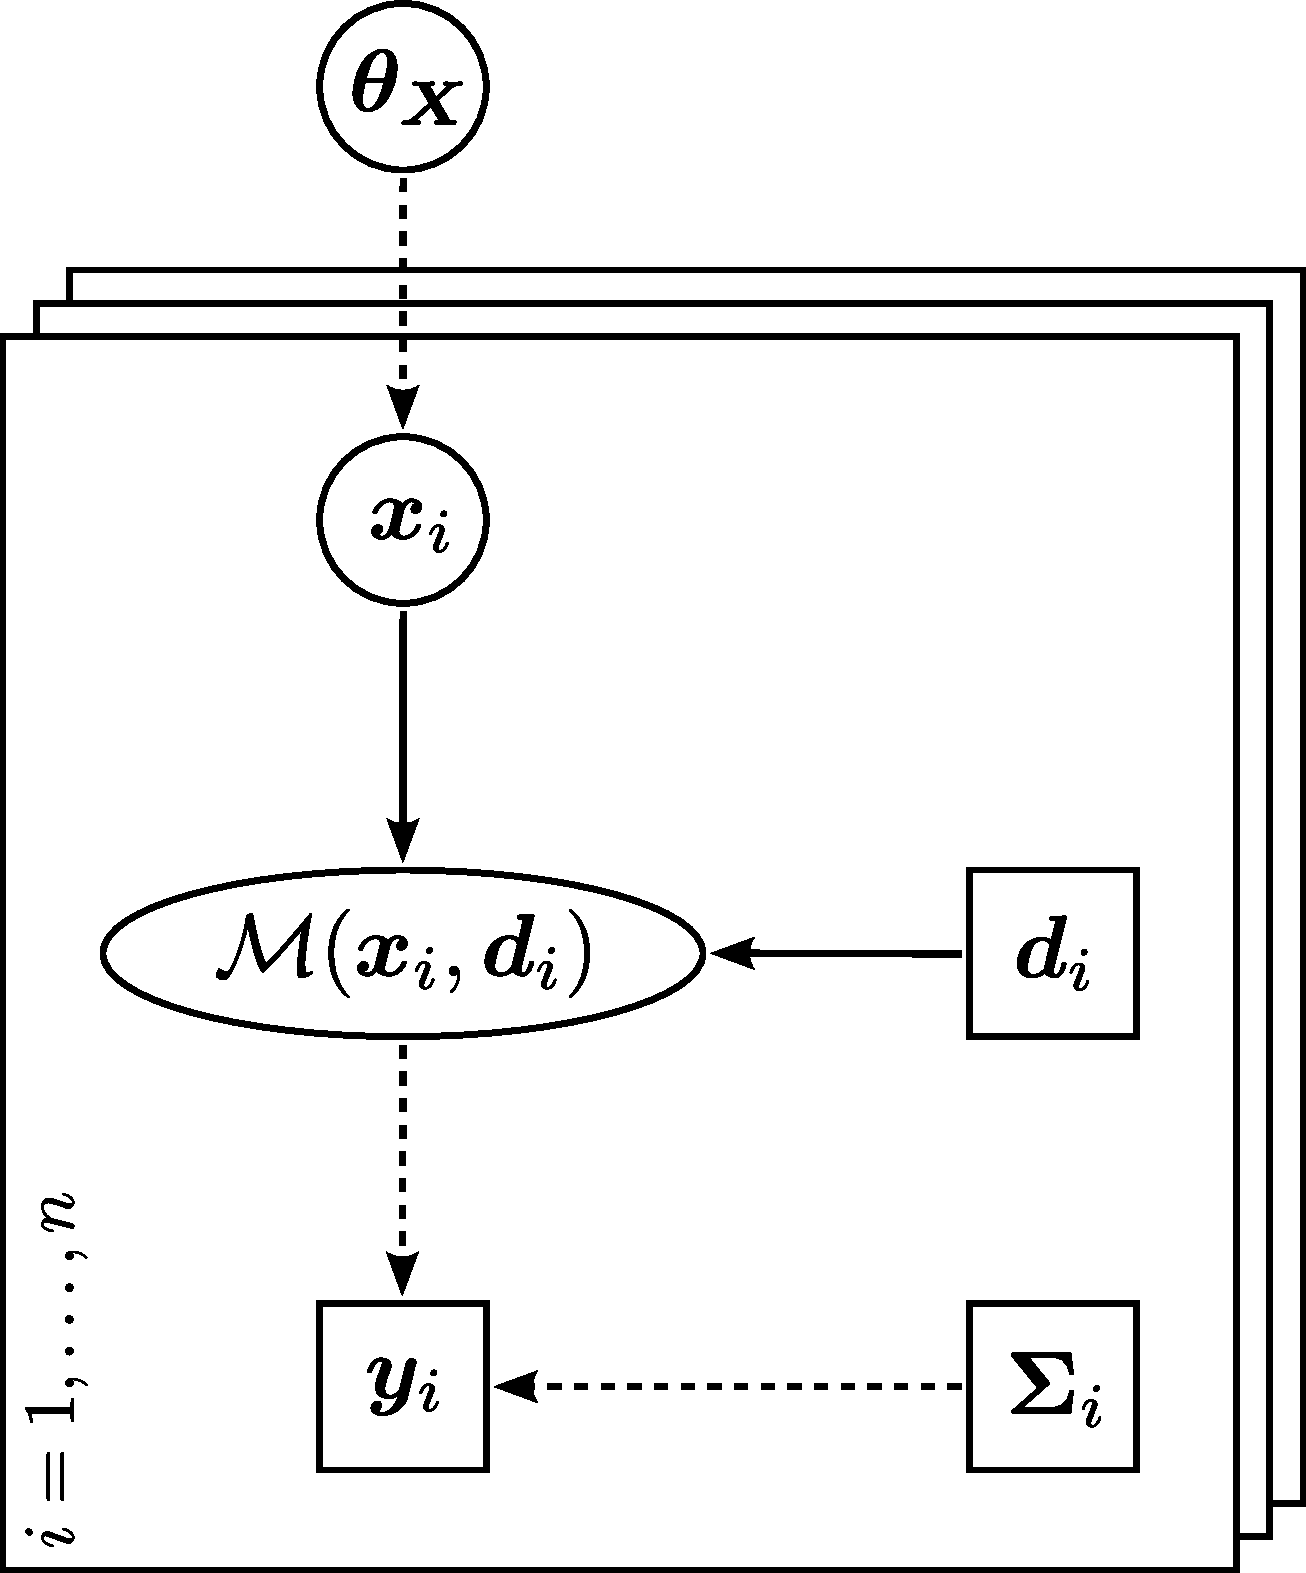
\includegraphics[width=\PEMdagWidth]{fig_PEM_DAG_ProbabilisticInversion}
    \caption{Probabilistic inversion.}
    \label{fig:PEM:DAG:ProbInv}
  \end{subfigure}%
  \begin{subfigure}[b]{0.33\textwidth}
    \centering
    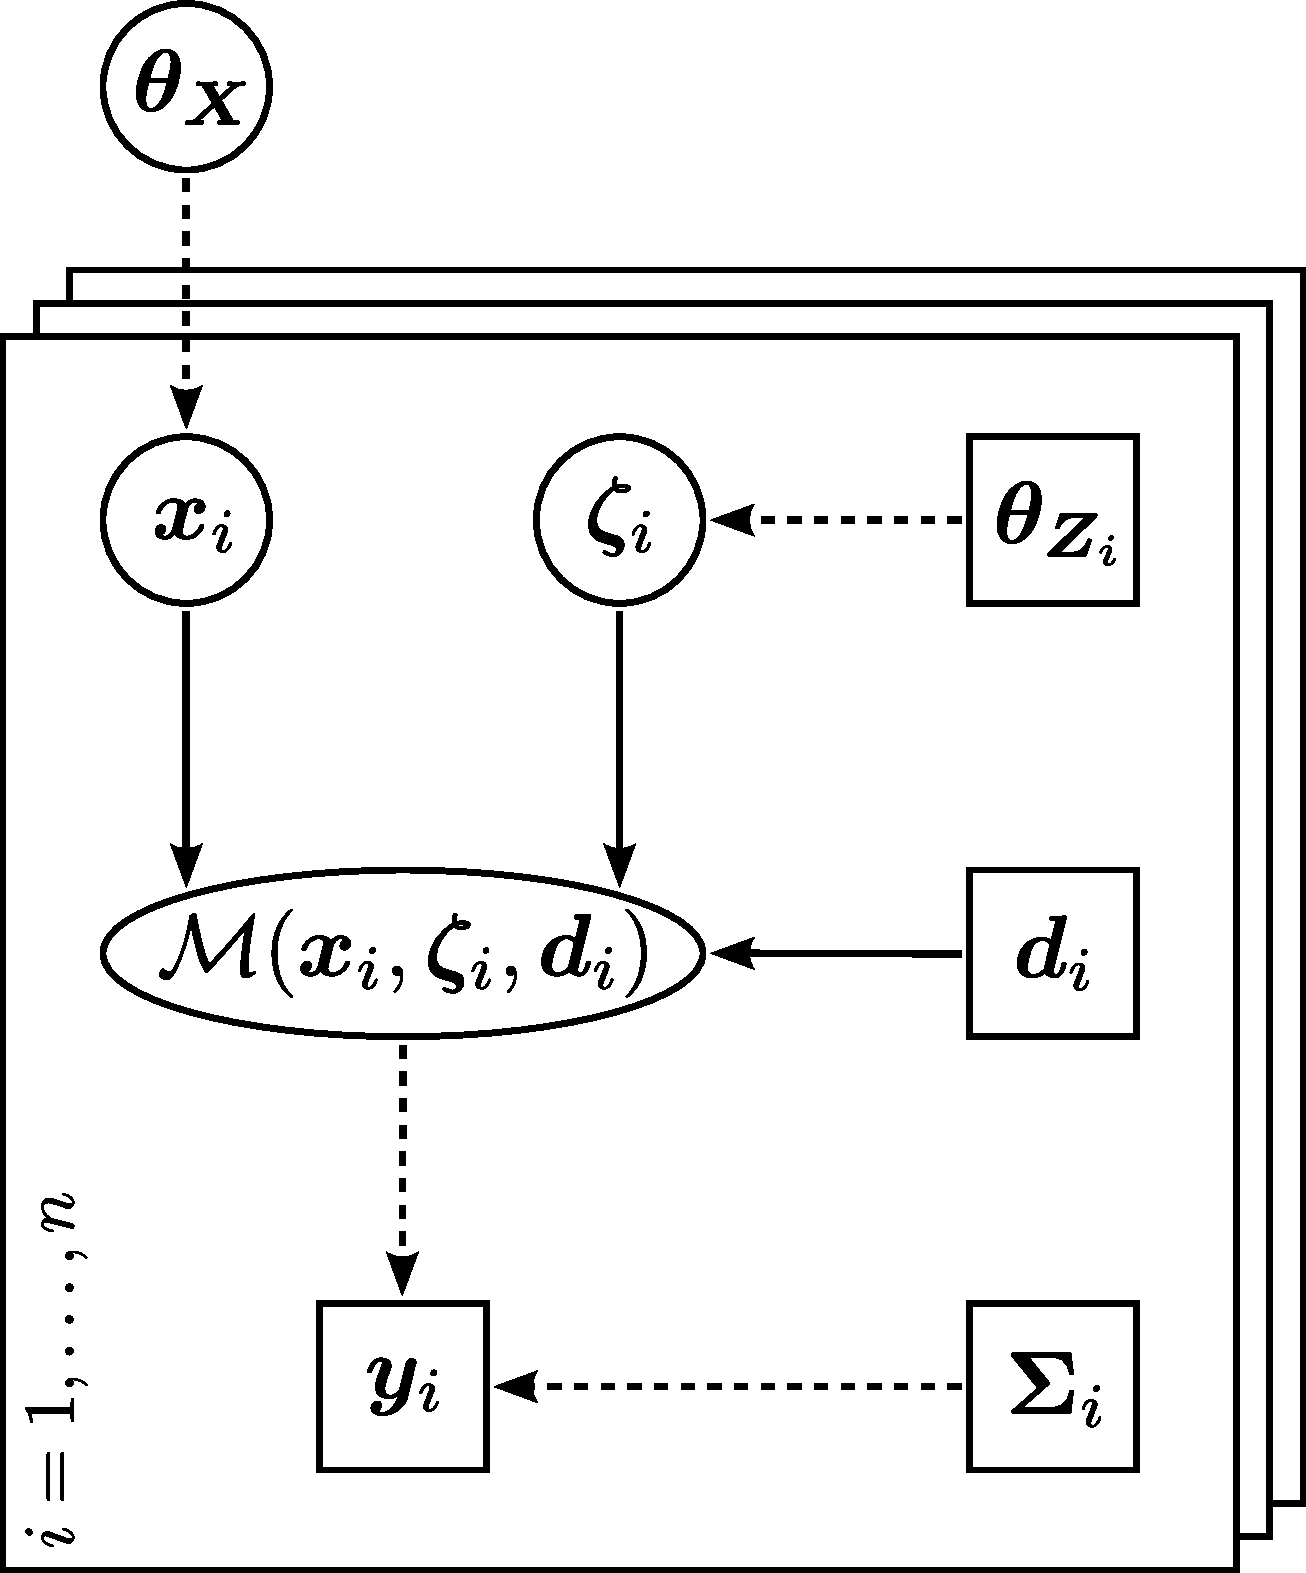
\includegraphics[width=\PEMdagWidth]{fig_PEM_DAG_AdditionalPrescription}
    \caption{Additional nuisance.}
    \label{fig:PEM:DAG:AddPres}
  \end{subfigure}%
  \caption[Various DAGs]{Various DAGs.
           Simple inversion, i.e.\ the estimation of an unknown \(\bm{m}\), is visualized in \subref{fig:PEM:DAG:SimpleInv},
           whereas \subref{fig:PEM:DAG:ProbInv} shows a DAG of probabilistic inversion, i.e.\ the inference of \(\bm{\theta}_{\bm{X}}\) that governs the variability  of experiment-specific \(\bm{x}_i\).
           An upgrade of probabilistic inversion, where a prescribed uncertainty has been introduced in nuisance variables \(\bm{\zeta}_i\), is depicted in \subref{fig:PEM:DAG:AddPres}.
           }
  \label{fig:PEM:DAG:Additional}
\end{figure}
%%%%%%%%%%%%%%%%%%%%%%%%%%%%%%%%%%%%%%%%
\par % GENERIC PROBABILISTIC INVERSION %
%%%%%%%%%%%%%%%%%%%%%%%%%%%%%%%%%%%%%%%%
The problem that we call probabilistic inversion shall not be confused with the identically named problem
of finding an input distribution of a forward model given its output distribution \cite{Inversion:Kraan2005,Inversion:Du2006}.
% PLACEMENT & CRITICISM 
Commonly engineering applications do not allow to exercise this type of uncertainty backpropagation.
The amount and structure of the data being available do not permit to fully specify a response distribution while expert knowledge refers to physical parameters instead.
%%%%%%%%%%%%%%%%%%%%%%%%%%%%%%%%
\par % PROBABILISTIC INVERSION %
%%%%%%%%%%%%%%%%%%%%%%%%%%%%%%%%
At this point we have a closer look at probabilistic inversion.
It results from removing the forward model inputs \(\bm{m}\) and \(\tuple{\bm{\zeta}_i}\) from the overall system \cref{eq:PEM:Multilevel:Model}
and from declaring \(\bm{\theta}_{\bm{X}}\) as QoI and \(\tuple{\bm{x}_i}\) as nuisance variables.
% MULTILEVEL MODEL
For the sake of completeness we summarize the associated multilevel model as
\begin{subequations} \label{eq:PEM:ProbInv:Model}
  \begin{align}
    (\bm{Y}_i \cond \bm{x}_i) &\sim f_{\bm{E}} \big( \bm{y}_i-\mathcal{M}(\bm{x}_i,\bm{d}_i) \distparam \bm{\Sigma}_i \big), \label{eq:PEM:ProbInv:Model:Data}\\
    (\bm{X}_i \cond \bm{\theta}_{\bm{X}} ) &\sim f_{\bm{X} \cond \bm{\Theta}_{\bm{X}}} (\bm{x}_i \cond \bm{\theta}_{\bm{X}}), \label{eq:PEM:ProbInv:Model:StructuralPrior}\\
    \bm{\Theta}_{\bm{X}} &\sim \pi_{\bm{\Theta}_{\bm{X}}} (\bm{\theta}_{\bm{X}}). \label{eq:PEM:ProbInv:Model:Hyperprior}
  \end{align}
\end{subequations}
% JOINT POSTERIOR
Joint Bayesian inference is accomplished by conditioning on the realized data \(\tuple{\bm{y}_i}\).
Up to a normalization factor, according to Bayes' law the posterior density is given as
\begin{equation} \label{eq:PEM:ProbInv:JointPosterior}
  \pi \big( \tuple{\bm{x}_i},\bm{\theta}_{\bm{X}} \cond \tuple{\bm{y}_i} \big)
  \propto \left( \prod\limits_{i=1}^n f_{\bm{E}} \big( \bm{y}_i-\mathcal{M}(\bm{x}_i,\bm{d}_i) \distparam \bm{\Sigma}_i \big) \right)
  \left( \prod\limits_{i=1}^n f_{\bm{X} \cond \bm{\Theta}_{\bm{X}}} (\bm{x}_i \cond \bm{\theta}_{\bm{X}}) \right)  \pi_{\bm{\Theta}_{\bm{X}}}(\bm{\theta}_{\bm{X}}).
\end{equation}
\par % MARGINAL PROBLEM
Equivalent to integrating out nuisance \(\tuple{\bm{x}_i}\) from the joint posterior \cref{eq:PEM:ProbInv:JointPosterior} as in \cref{eq:PEM:Multilevel:Inference:MarginalizedPosterior1},
one can base inference of \(\bm{\theta}_{\bm{X}}\) on an inherently marginal problem formulation \cite{Multilevel:Rocquigny2009,Uncertainty:Rocquigny2012}.
% MARGINALIZED LIKELIHOOD
Similar to \cref{eq:PEM:Multilevel:Marginal:Marginalization,eq:PEM:Multilevel:Marginal:Likelihood} the marginalized likelihood function for that case is derived as
\begin{equation} \label{eq:PEM:ProbInv:MarginalizedLikelihood}
  \mathcal{L} \big( \bm{\theta}_{\bm{X}} \distparam \tuple{\bm{y}_i} \big)
  = f \big( \tuple{\bm{y}_i} \cond \bm{\theta}_{\bm{X}} \big)
  = \prod\limits_{i=1}^n \int\limits_{\mathcal{D}_{\bm{x}}} f_{\bm{E}} \big( \bm{y}_i-\mathcal{M}(\bm{x}_i,\bm{d}_i) \distparam \bm{\Sigma}_i \big)
  \, f_{\bm{X} \cond \bm{\Theta}_{\bm{X}}} (\bm{x}_i \cond \bm{\theta}_{\bm{X}}) \, \mathrm{d} \bm{x}_i.
\end{equation}
% MARGINAL POSTERIOR
With the marginalized likelihood function \cref{eq:PEM:ProbInv:MarginalizedLikelihood} and the marginal prior distribution \cref{eq:PEM:ProbInv:Model:Hyperprior},
the unscaled version of the marginal posterior reduces to
\begin{equation} \label{eq:PEM:ProbInv:MarginalPosterior}
  \pi \big( \bm{\theta}_{\bm{X}} \cond \tuple{\bm{y}_i} \big) \propto \mathcal{L} (\bm{\theta}_{\bm{X}} \distparam \tuple{\bm{y}_i}) \, \pi_{\bm{\Theta}_{\bm{X}}} (\bm{\theta}_{\bm{X}}).
\end{equation}
% NUMERICAL EFFICIENCY
Exemplary comparisons of the numerical efficiency for sampling joint posteriors of the form \cref{eq:PEM:ProbInv:JointPosterior}
and marginal posteriors of the form \cref{eq:PEM:ProbInv:MarginalPosterior} are found in \cite{Nagel:IPW2013:Proc,Multilevel:Ballesteros2014:Proc}.
%%%%%%%%%%%%%%%%%%%%%%%%%%
\par % TWO-STAGE METHODS %
%%%%%%%%%%%%%%%%%%%%%%%%%%
Approximate \textit{two-stage approaches} have been proposed for inferring aleatory parameter variability in inverse problems,
e.g.\ the context of random fields \cite{PCE:Desceliers2006,PCE:Desceliers2007,Multilevel:Mehrez2012:II,Multilevel:Debruyne2015}.
In the first stage \(n\) separate inverse problems are solved, i.e.\ for each experiment \(i = 1,\ldots,n\) an estimator \(\hat{\bm{x}}_i\) of the realization \(\bm{x}_i\) is computed.
As a second step the hyperparameters \(\bm{\theta}_{\bm{X}}\) are identified by statistical analysis of the estimates \(\tuple{\hat{\bm{x}}_i}\).
% CRITICISM
However, two-stage methods suffer from the dependence on a sufficient amount of data available for both of the stages
and their tendency to overestimate second-order central moments \cite{Multilevel:Davidian2003,Multilevel:Banks2012}.
Those issues are due to a fundamental inconsistency in treating epistemic and aleatory uncertainty.
%%%%%%%%%%%%%%%%%%%%%%%%%%%%%%%%%%%%%%%%%
\par % HIERARCHICAL (& EMPIRICAL BAYES) %
%%%%%%%%%%%%%%%%%%%%%%%%%%%%%%%%%%%%%%%%%
Classical inverse problems are sometimes phrased within a hierarchical frame \cite{Multilevel:Malinverno2004,Inversion:Wang2005:b}.
Formally this is a special case of probabilistic inversion with \(n = 1\).
% PRIOR DECOMPOSITION
The intermediate unknowns \(\bm{x}_1\) are commonly the QoI in this type of \textit{hierarchical inversion}.
Their prior \(\pi(\bm{x}_1) = \int f_{\bm{X} \cond \bm{\Theta}_{\bm{X}}} (\bm{x}_1 \cond \bm{\theta}_{\bm{X}}) \, \pi_{\bm{\Theta}_{\bm{X}}}(\bm{\theta}_{\bm{X}}) \, \mathrm{d} \bm{\theta}_{\bm{X}}\)
decomposes into a conditional distribution \(f_{\bm{X} \cond \bm{\Theta}_{\bm{X}}} (\bm{x}_1 \cond \bm{\theta}_{\bm{X}})\) and a marginal one \(\pi_{\bm{\Theta}_{\bm{X}}} (\bm{\theta}_{\bm{X}})\).
% NO ALEATORY VARIABILITY
However, other than in probabilistic inversion, \cref{eq:PEM:ProbInv:Model:StructuralPrior} is not interpreted as aleatory variability.
% INTERPRETATION: INCOMPLETELY SPECIFIED / UNCERTAIN PRIOR
Instead it can be viewed as leaving the prior for \(\bm{x}_1\) incompletely specified \cite{Multilevel:Malinverno2004},
i.e.\ relaxing the assumption of a parametric prior \(\pi(\bm{x}_1 \distparam \bm{\theta}_{\bm{X}}) = f_{\bm{X} \cond \bm{\Theta}_{\bm{X}}} (\bm{x}_1 \cond \bm{\theta}_{\bm{X}})\) for a specific value \(\bm{\theta}_{\bm{X}}\).
% INTERPRETATION: REGULARIZATION INFORMED BY THE DATA
Alternatively \cref{eq:PEM:ProbInv:JointPosterior} suggests that the prior hyperparameters \(\bm{\theta}_{\bm{X}}\) can be estimated along with \(\bm{x}_1\).
The prior in this case is given as \(\pi(\bm{x}_1,\bm{\theta}_{\bm{X}}) = f_{\bm{X} \cond \bm{\Theta}_{\bm{X}}} (\bm{x}_1 \cond \bm{\theta}_{\bm{X}}) \, \pi_{\bm{\Theta}_{\bm{X}}}(\bm{\theta}_{\bm{X}})\).
For solving ill-posed problems this can be seen as an automatic determination of the regularization parameters \cite{Inversion:Wang2005:b}.